\documentclass[a4paper,11pt,exos]{nsi} 

\usepackage{pifont}
\usepackage{fontawesome5}
\geometry{margin=2cm}

\pagestyle{empty}

\begin{document}
\classe{\premiere spé}
\titre{Corrigé de l'interro 2 - A}
\maketitle

\exo{}
\dleft{8cm}{
    \textcolor{UGLiBlue}{Résoudre graphiquement le système suivant : $$\left\{
			\begin{array}{l}
				\ y=-2x+3 \\
				\ x-2y=4 \\
			\end{array} \right.$$}
    \begin{tabbing}
        $x-2y=4 \quad$ \=   $\iff \quad -2y=-x+4$\\[.5em]
        \>  $\iff\quad y=\dfrac{-1}{-2}x+\dfrac{4}{-2}$\\[.5em]
        \>  $\iff\quad y=\dfrac{1}{2}x-2$
    \end{tabbing}
            On trace $(d_1)$ la droite d'équation $y=-2x+3$ et $(d_2)$ la droite d'équation $y=\dfrac{1}{2}x-2$.\\
            $(d_1)$ et $(d_2)$ sont séantes au point de coordonnées $(2\ ;-1)$.\\
            Donc le couple solution du système est $(2\ ;-1)$.
    }
{
    \def\xmin{-5}	\def\xmax{7}	\def\ymin{-5}	\def\ymax{7}
    \begin{tikzpicture}[scale = .7]
        \draw[fill=white](\xmin,\ymin) rectangle (\xmax,\ymax);
        \reperevl{\xmin}{\ymin}{\xmax}{\ymax}
        \clip (\xmin,\ymin) rectangle (\xmax,\ymax);
        \draw[UGLiOrange,domain=\xmin:\xmax,samples=2,variable=\x] plot ({\x},{-2*\x+3});
        \draw[UGLiDarkGreen,domain=\xmin:\xmax,samples=2,variable=\x] plot ({\x},{.5*\x-2});
        \node[UGLiOrange] () 	at 	(4.5,-4.5){$(d_1)$};
        \node[UGLiDarkGreen]() at 	(6,1.5){$(d_2)$};
        \draw (2,-1)\ball;
    \end{tikzpicture}
}

\exo{}
\textcolor{UGLiBlue}{Sophia a travailé durant l'été 45 jours dans deux entreprises. Dans la première, elle a gagné 85 € par jour et dans la deuxième, 72 € par jour. Au total, elle a gagné 3487 €.\\
On cherche à savoir le nombre de jours pendant lesquels Sophia a travaillé dans chaque entreprise.\\[.5em]
Modéliser cette situation par un système. \textit{On ne demande pas de le résoudre}\\}

On appelle $x$ le nombre de jours pendant lesquels Sophia a travaillé dans la première entreprise et $y$ le nombre de jours pendant lesquels elle a travaillé dans la deuxième.\\[.5em]
Sophia a travailé 45 jours dans deux entreprises ; donc $\quad x+y=45$.\\[.5em]
Au total, Sophia a gagné 3487 € ; donc $\quad 85x+72y=3487$.\\[.5em]
Cette situation peut donc être modélisée par le système :
$$\left\{
			\begin{array}{l}
				\ x+y=45 \\
				\ 85x+72y=3487 \\
			\end{array} \right.$$



\exo{}
%\begin{multicols}{2}
    \begin{enumerate}
        \item \textcolor{UGLiBlue}{Résoudre le système suivant par substitution : $\left\{
			\begin{array}{l}
				\ 3x+y=4 \\
				\ -2x+3y=-10 \\
			\end{array} \right.$}

            Soit $(x\ ;y)$ un couple de réels.
            \begin{tabbing}
                $\left\{
                    \begin{array}{l}
                    \ 3x+y=4 \\
                    \ -2x+3y=-10 \\
                \end{array} \right. \quad$
                \= $\iff \quad \left\{
                    \begin{array}{l}
                    \ y=4-3x \\
                    \ -2x+3y=-10 \\
                \end{array} \right.$\\[1em]
                
                \>  $\iff \quad \left\{
                    \begin{array}{l}
                    \ y=4-3x \\
                    \ -2x+3(4-3x)=-10 \\
                \end{array} \right.$\\[1em]
        
                \>  $\iff \quad \left\{
                    \begin{array}{l}
                    \ y=4-3x \\
                    \ -2x+12-9x=-10 \\
                \end{array} \right.$\\[1em]
        
                \>  $\iff \quad \left\{
                    \begin{array}{l}
                    \ y=4-3x \\
                    \ -11x=-22 \\
                \end{array} \right.$\\[1em]
        
                \>  $\iff \quad \left\{
                    \begin{array}{l}
                    \ y=4-3x \\
                    \ x=2 \\
                \end{array} \right.$\\[1em]
        
                \>  $\iff \quad \left\{
                    \begin{array}{l}
                    \ y=4-3\times 2 \\
                    \ x=2 \\
                \end{array} \right.$\\[1em]
        
                \>  $\iff \quad \left\{
                    \begin{array}{l}
                    \ y=-2 \\
                    \ x=2 \\
                \end{array} \right.$
            \end{tabbing}
        D'où $\mathcal{S}_1=\left\{(2\ ;-2)\right\}$.

        \item \textcolor{UGLiBlue}{Résoudre le système suivant par combinaison linéaire : $\left\{
			\begin{array}{l}
				\ 3x-4y=6 \\
				\ -5x+2y=4 \\
			\end{array} \right.$}

    Soit $(x\ ;y)$ un couple de réels.
    \begin{tabbing}
        $\left\{
            \begin{array}{l}
            \ 3x-4y=6 \\
			\ -5x+2y=4 \\
        \end{array} \right. \quad$
        \= $\iff \quad \left\{
            \begin{array}{l}
            \ 3x-4y=6 \\
            \ 2(-5x+2y)=2\times 4 \\
        \end{array} \right.$\\[1em]
        
        \>  $\iff \quad \left\{
            \begin{array}{l}
            \ 3x-4y=6 \\
            \ -10x+4y=8 \\
        \end{array} \right.$\\[1em]

        \>  $\iff \quad \left\{
            \begin{array}{l}
            \ 3x-4y=6 \\
            \ 3x-10x-4y+4y=6+8 \\
        \end{array} \right.$\\[1em]

        \>  $\iff \quad \left\{
            \begin{array}{l}
            \ 3x-4y=6 \\
            \ -7x=14 \\
        \end{array} \right.$\\[1em]

        \>  $\iff \quad \left\{
            \begin{array}{l}
            \ 3x-4y=6 \\
            \ x=-2 \\
        \end{array} \right.$\\[1em]

        \>  $\iff \quad \left\{
            \begin{array}{l}
            \ 3\times (-2)-4y=6 \\
            \ x=-2 \\
        \end{array} \right.$\\[1em]

        \>  $\iff \quad \left\{
            \begin{array}{l}
            \ -6-4y=6 \\
            \ x=-2 \\
        \end{array} \right.$\\[1em]

        \>  $\iff \quad \left\{
            \begin{array}{l}
            \ -4y=12 \\
            \ x=-2 \\
        \end{array} \right.$\\[1em]

        \>  $\iff \quad \left\{
            \begin{array}{l}
            \ y=-3 \\
            \ x=-2 \\
        \end{array} \right.$\\[1em]
    \end{tabbing}
    D'où $\mathcal{S}_2=\left\{(-2\ ;-3)\right\}$.
\end{enumerate}


%\newpage
\exo{}
\textcolor{UGLiBlue}{Soit $x$ un nombre réel strictement supérieur à $1$.\\
$A, B$ et $C$ sont trois points tels que $\quad AB=4x+3$, $\quad BC=3(x-1)\quad$ et $\quad AC=5x+1$.\\
On considère le point $D$ tel que $ABCD$ est un parallélogramme.}
\begin{enumerate}
	\item 	\textcolor{UGLiBlue}{Faire un schéma codé.}
	\begin{center}
        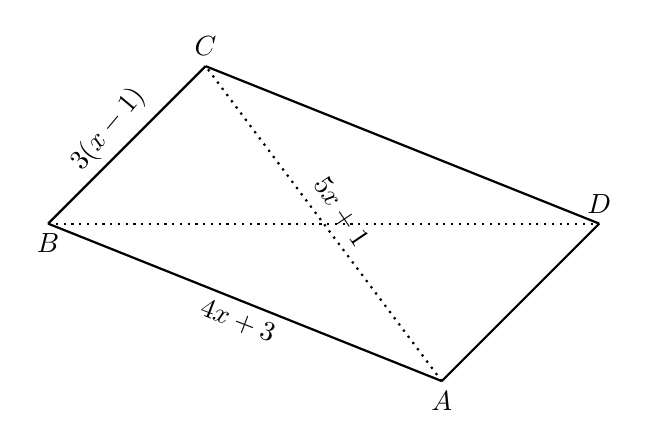
\begin{tikzpicture}[scale=1]
            \coordinate (A) at (5,0);
            \coordinate (B) at (0,2);
            \coordinate (D) at (7,2);
            \coordinate (C) at (2,4);		
            \draw[thick] 	(A) node[below]{$A$} -- node[midway,rotate=-21,below]{$4x+3$} 	
            (B) node[below]{$B$};
            \draw[thick] (C) node[above]{$C$} -- 
            (D) node[above]{$D$};
            \draw[thick,dotted] (A) -- node[midway,rotate=-56,above]{$5x+1$} (C);
            \draw[thick,dotted] (B) -- (D);
            \draw [thick] (B) -- node[midway,rotate=50,above]{$3(x-1)$} (C);
            \draw [thick] (A) -- (D);
        \end{tikzpicture}
    \end{center}
	\item   \textcolor{UGLiBlue}{Résoudre l'équation $\quad 25x^2+10x+1=25x^2+6x+18$.}\\[.5em]
	Soit $x\in\oio{1}{+\infty}$.
    \begin{tabbing}
        $25x^2+10x+1=25x^2+6x+18\quad$  \=  $\iff\quad 10x+1=6x+18$\\
        \>  $\iff\quad 4x=17$\\
        \>  $\iff\quad x=\dfrac{17}{4}$\\
        \>  $\iff\quad x=4,25$
    \end{tabbing}
    D'où $\mathcal{S}=\left\{\dfrac{17}{4}\right\}$
	\item 	\textcolor{UGLiBlue}{Démontrer que le parallélogramme $ABCD$ est un rectangle si, et seulement si $\quad x=\dfrac{17}{4}$.\\
	\textit{Raisonner par équivalences.}}
    \begin{tabbing}
        $ABCD$ est un rectangle $\quad$ \= $\iff\quad ABC$ est rectangle en $B$\\
        \>  $\iff\quad AC^2=AB^2+BC^2$\\
        \>  $\phantom{\iff} \quad$ \textit{d'après le théorème de Pythagore et sa réciproque}\\
        \> $\iff\quad (5x+1)^2=(4x+3)^2+\left(3(x-1)\right)^2$\\
        \> $\iff\quad (5x)^2+2\times 5x\times 1+1^2=(4x)^2+2\times 4x\times 3+3^2+(3x-3)^2$\\
        \> $\iff\quad 25x^2+10+1=16x^2+24x+9+(3x)^2-2\times 3x\times 3+3^2$\\
        \> $\iff\quad 25x^2+10+1=16x^2+24x+9+9x^2-18x+9$\\
        \> $\iff\quad 25x^2+10+1=25x^2+6x+18$\\[0.5em]
        \> $\iff\quad x=\dfrac{17}{4}\quad$\textit{d'après la question précédente.}
    \end{tabbing}	
  
	\item	 \textcolor{UGLiBlue}{Quelle est alors la longueur $BD$ ?}\\[.5em]
	Si $x=\dfrac{17}{4}$, alors $ABCD$ est une rectangle et ses diagonales sont de même longueur. On a donc :
    \begin{tabbing}
        On a donc : $\quad BD$    \=$=AC$\\[.5em]
        \>  $=5\times \dfrac{17}{4}+1$\\[.5em]
        \>  $=\dfrac{85}{4}+\dfrac{4}{4}$\\[.5em]
        \>  $=\dfrac{89}{4}$\\[.5em]
        \>  $=22,25$
    \end{tabbing}
\end{enumerate}


\newpage

\setcounter{section}{0}



\classe{\premiere spé}
\titre{Corrigé de l'interro 2 - B}
\maketitle
\exo{}
\dleft{8cm}{
    \textcolor{UGLiBlue}{Résoudre graphiquement le système suivant : $$\left\{
			\begin{array}{l}
				\ y=2x-1 \\
				\ x+2y=8 \\
			\end{array} \right.$$}

    \begin{tabbing}
        $x+2y=8 \quad$ \=   $\iff \quad 2y=-x+8$\\[.5em]
        \>  $\iff\quad y=\dfrac{-1}{2}x+\dfrac{8}{2}$\\[.5em]
        \>  $\iff\quad y=-\dfrac{1}{2}x+4$
    \end{tabbing}
            On trace $(d_1)$ la droite d'équation $y=2x-1$ et $(d_2)$ la droite d'équation $y=-\dfrac{1}{2}x+4$.\\
            $(d_1)$ et $(d_2)$ sont séantes au point de coordonnées $(2\ ;3)$.\\
            Donc le couple solution du système est $(2\ ;3)$.
}
{
    \def\xmin{-5}	\def\xmax{7}	\def\ymin{-5}	\def\ymax{7}
    \begin{tikzpicture}[scale = .7]
        \draw[fill=white](\xmin,\ymin) rectangle (\xmax,\ymax);
        \reperevl{\xmin}{\ymin}{\xmax}{\ymax}
        \clip (\xmin,\ymin) rectangle (\xmax,\ymax);
        \draw[UGLiOrange,domain=\xmin:\xmax,samples=2,variable=\x] plot ({\x},{2*\x-1});
        \draw[UGLiDarkGreen,domain=\xmin:\xmax,samples=2,variable=\x] plot ({\x},{-.5*\x+4});
        \node[UGLiOrange] () 	at 	(-2.5,-4.5){$(d_1)$};
        \node[UGLiDarkGreen]() at 	(-4,5.5){$(d_2)$};
        \draw (2,3)\ball ;
    \end{tikzpicture}
}

\exo{} 
\textcolor{UGLiBlue}{Sophia a travailé durant l'été 52 jours dans deux entreprises. Dans la première, elle a gagné 65 € par jour et dans la deuxième, 82 € par jour. Au total, elle a gagné 3652 €.\\
On cherche à savoir le nombre de jours pendant lesquels Sophia a travaillé dans chaque entreprise.\\[.5em]
Modéliser cette situation par un système. \textit{On ne demande pas de le résoudre.}}\\

On appelle $x$ le nombre de jours pendant lesquels Sophia a travaillé dans la première entreprise et $y$ le nombre de jours pendant lesquels elle a travaillé dans la deuxième.\\[.5em]
Sophia a travailé 52 jours dans deux entreprises ; donc $\quad x+y=52$.\\[.5em]
Au total, Sophia a gagné 3652 € ; donc $\quad 65x+82y=3652$.\\[.5em]
Cette situation peut donc être modélisée par le système :
$$\left\{
			\begin{array}{l}
				\ x+y=52 \\
				\ 65x+82y=3652 \\
			\end{array} \right.$$

\exo{}
%\begin{multicols}{2}
    \begin{enumerate}
        \item \textcolor{UGLiBlue}{Résoudre le système suivant par substitution : $\left\{
			\begin{array}{l}
				\ x-2y=5 \\
				\ 3x+2y=7 \\
			\end{array} \right.$}
        
    Soit $(x\ ;y)$ un couple de réels.
            \begin{tabbing}
                $\left\{
                    \begin{array}{l}
                    \ x-2y=5 \\
                    \ 3x+2y=7 \\
                \end{array} \right. \quad$
                \= $\iff \quad \left\{
                    \begin{array}{l}
                    \ x=2y+5 \\
                    \ 3x+2y=7  \\
                \end{array} \right.$\\[1em]
                
                \>  $\iff \quad \left\{
                    \begin{array}{l}
                    \ x=2y+5 \\
                    \ 3(2y+5)+2y=7\\
                \end{array} \right.$\\[1em]

                \>  $\iff \quad \left\{
                    \begin{array}{l}
                    \ x=2y+5 \\
                    \ 6y+15+2y=7\\
                \end{array} \right.$\\[1em]

                \>  $\iff \quad \left\{
                    \begin{array}{l}
                    \ x=2y+5 \\
                    \ 8y=-8\\
                \end{array} \right.$\\[1em]

                \>  $\iff \quad \left\{
                    \begin{array}{l}
                    \ x=2y+5 \\
                    \ y=-1\\
                \end{array} \right.$\\[1em]

                \>  $\iff \quad \left\{
                    \begin{array}{l}
                    \ x=2\times (-1)+5 \\
                    \ y=-1\\
                \end{array} \right.$\\[1em]

                \>  $\iff \quad \left\{
                    \begin{array}{l}
                    \ x=3 \\
                    \ y=-1\\
                \end{array} \right.$
            \end{tabbing}
            D'où $\mathcal{S}_1=\left\{(3\ ;-1)\right\}$.
        \item \textcolor{UGLiBlue}{Résoudre le système suivant par combinaison linéaire : $\left\{
			\begin{array}{l}
				\ 3x-4y=5 \\
				\ -6x+5y=-4 \\
			\end{array} \right.$}
        
        Soit $(x\ ;y)$ un couple de réels.
            \begin{tabbing}
                $\left\{
                    \begin{array}{l}
                    \ 3x-4y=5 \\
                    \ -6x+5y=-4 \\
                \end{array} \right. \quad$
                \= $\iff \quad \left\{
                    \begin{array}{l}
                    \ 2(3x-4y)=2\times 5 \\
                    \ -6x+5y=-4 \\
                \end{array} \right.$\\[1em]
                
                \>  $\iff \quad \left\{
                    \begin{array}{l}
                    \ 6x-8y=10 \\
                    \ -6x+5y=-4 \\
                \end{array} \right.$\\[1em]

                \>  $\iff \quad \left\{
                    \begin{array}{l}
                    \ 6x-8y=10 \\
                    \ 6x-6x-8y+5y=10-4 \\
                \end{array} \right.$\\[1em]

                \>  $\iff \quad \left\{
                    \begin{array}{l}
                    \ 6x-8y=10 \\
                    \ -3y=6 \\
                \end{array} \right.$\\[1em]

                \>  $\iff \quad \left\{
                    \begin{array}{l}
                    \ 6x-8y=10 \\
                    \ y=-2 \\
                \end{array} \right.$\\[1em]

                \>  $\iff \quad \left\{
                    \begin{array}{l}
                    \ 6x-8\times(-2)=10 \\
                    \ y=-2 \\
                \end{array} \right.$\\[1em]

                \>  $\iff \quad \left\{
                    \begin{array}{l}
                    \ 6x+16=10 \\
                    \ y=-2 \\
                \end{array} \right.$\\[1em]

                \>  $\iff \quad \left\{
                    \begin{array}{l}
                    \ 6x=-6\\
                    \ y=-2 \\
                \end{array} \right.$\\[1em]

                \>  $\iff \quad \left\{
                    \begin{array}{l}
                    \ x=-1\\
                    \ y=-2 \\
                \end{array} \right.$\\[1em]
            \end{tabbing}
            D'où $\mathcal{S}_2=\left\{(-1\ ;-2)\right\}$.
    \end{enumerate}
%\end{multicols}



%\newpage
\exo{}
\textcolor{UGLiBlue}{Soit $x$ un nombre réel strictement supérieur à $1$.\\
$A, B$ et $C$ sont trois points tels que $\quad AB=4x+3$, $\quad BC=3(x-1)\quad$ et $\quad AC=5x+1$.\\
On considère le point $D$ tel que $ABCD$ est un parallélogramme.}
\begin{enumerate}
	\item 	\textcolor{UGLiBlue}{Faire un schéma codé.}
	\begin{center}
        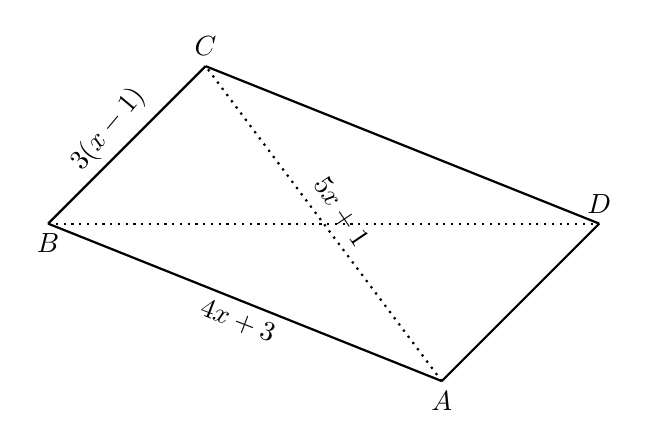
\begin{tikzpicture}[scale=1]
            \coordinate (A) at (5,0);
            \coordinate (B) at (0,2);
            \coordinate (D) at (7,2);
            \coordinate (C) at (2,4);		
            \draw[thick] 	(A) node[below]{$A$} -- node[midway,rotate=-21,below]{$4x+3$} 	
            (B) node[below]{$B$};
            \draw[thick] (C) node[above]{$C$} -- 
            (D) node[above]{$D$};
            \draw[thick,dotted] (A) -- node[midway,rotate=-56,above]{$5x+1$} (C);
            \draw[thick,dotted] (B) -- (D);
            \draw [thick] (B) -- node[midway,rotate=50,above]{$3(x-1)$} (C);
            \draw [thick] (A) -- (D);
        \end{tikzpicture}
    \end{center}
	\item   \textcolor{UGLiBlue}{Résoudre l'équation $\quad 25x^2+10x+1=25x^2+6x+18$.}\\[.5em]
	Soit $x\in\oio{1}{+\infty}$.
    \begin{tabbing}
        $25x^2+10x+1=25x^2+6x+18\quad$  \=  $\iff\quad 10x+1=6x+18$\\
        \>  $\iff\quad 4x=17$\\
        \>  $\iff\quad x=\dfrac{17}{4}$\\
        \>  $\iff\quad x=4,25$
    \end{tabbing}
    D'où $\mathcal{S}=\left\{\dfrac{17}{4}\right\}$
	\item 	\textcolor{UGLiBlue}{Démontrer que le parallélogramme $ABCD$ est un rectangle si, et seulement si $\quad x=\dfrac{17}{4}$.\\
	\textit{Raisonner par équivalences.}}
    \begin{tabbing}
        $ABCD$ est un rectangle $\quad$ \= $\iff\quad ABC$ est rectangle en $B$\\
        \>  $\iff\quad AC^2=AB^2+BC^2$\\
        \>  $\phantom{\iff} \quad$ \textit{d'après le théorème de Pythagore et sa réciproque}\\
        \> $\iff\quad (5x+1)^2=(4x+3)^2+\left(3(x-1)\right)^2$\\
        \> $\iff\quad (5x)^2+2\times 5x\times 1+1^2=(4x)^2+2\times 4x\times 3+3^2+(3x-3)^2$\\
        \> $\iff\quad 25x^2+10+1=16x^2+24x+9+(3x)^2-2\times 3x\times 3+3^2$\\
        \> $\iff\quad 25x^2+10+1=16x^2+24x+9+9x^2-18x+9$\\
        \> $\iff\quad 25x^2+10+1=25x^2+6x+18$\\[0.5em]
        \> $\iff\quad x=\dfrac{17}{4}\quad$\textit{d'après la question précédente.}
    \end{tabbing}	
  
	\item	 \textcolor{UGLiBlue}{Quelle est alors la longueur $BD$ ?}\\[.5em]
	Si $x=\dfrac{17}{4}$, alors $ABCD$ est une rectangle et ses diagonales sont de même longueur. On a donc :
    \begin{tabbing}
        On a donc : $\quad BD$    \=$=AC$\\[.5em]
        \>  $=5\times \dfrac{17}{4}+1$\\[.5em]
        \>  $=\dfrac{85}{4}+\dfrac{4}{4}$\\[.5em]
        \>  $=\dfrac{89}{4}$\\[.5em]
        \>  $=22,25$
    \end{tabbing}
\end{enumerate}


\end{document}